%!TEX root = ../main.tex
\subsection{Copula robustness check}
\label{sub:05_robust}

This section provides an in-sample robustness check of how well the copula models can reproduce the threshold correlations and rolling correlations found in the dependence analysis of ARMA-GARCH residuals. By comparing simulated data from the copulas to the empirical data, we find that the main features are captured. However, we highlight that tail dependence is only reconstructed to a certain extent.

\subsubsection{Threshold correlations in constant copulas}
By simulating 250,000 weeks of shocks in the copula, and then transforming these shocks into standardized residuals for each of the factors, we can test the constant \textit{t} copula's ability to generate the threshold correlations in the ARMA-GARCH residuals.\footnote{This robustness check is inspired by \textcite{ChristoffersenLanglois2013}.} If a Student's \textit{t} copula specification reasonably well captures tail dependence, the threshold correlations from the empirical and the copula specification should align. The results are presented in~\autoref{fig:threshold_simulated1}.

\begin{figure}[!ht]
  \centering
  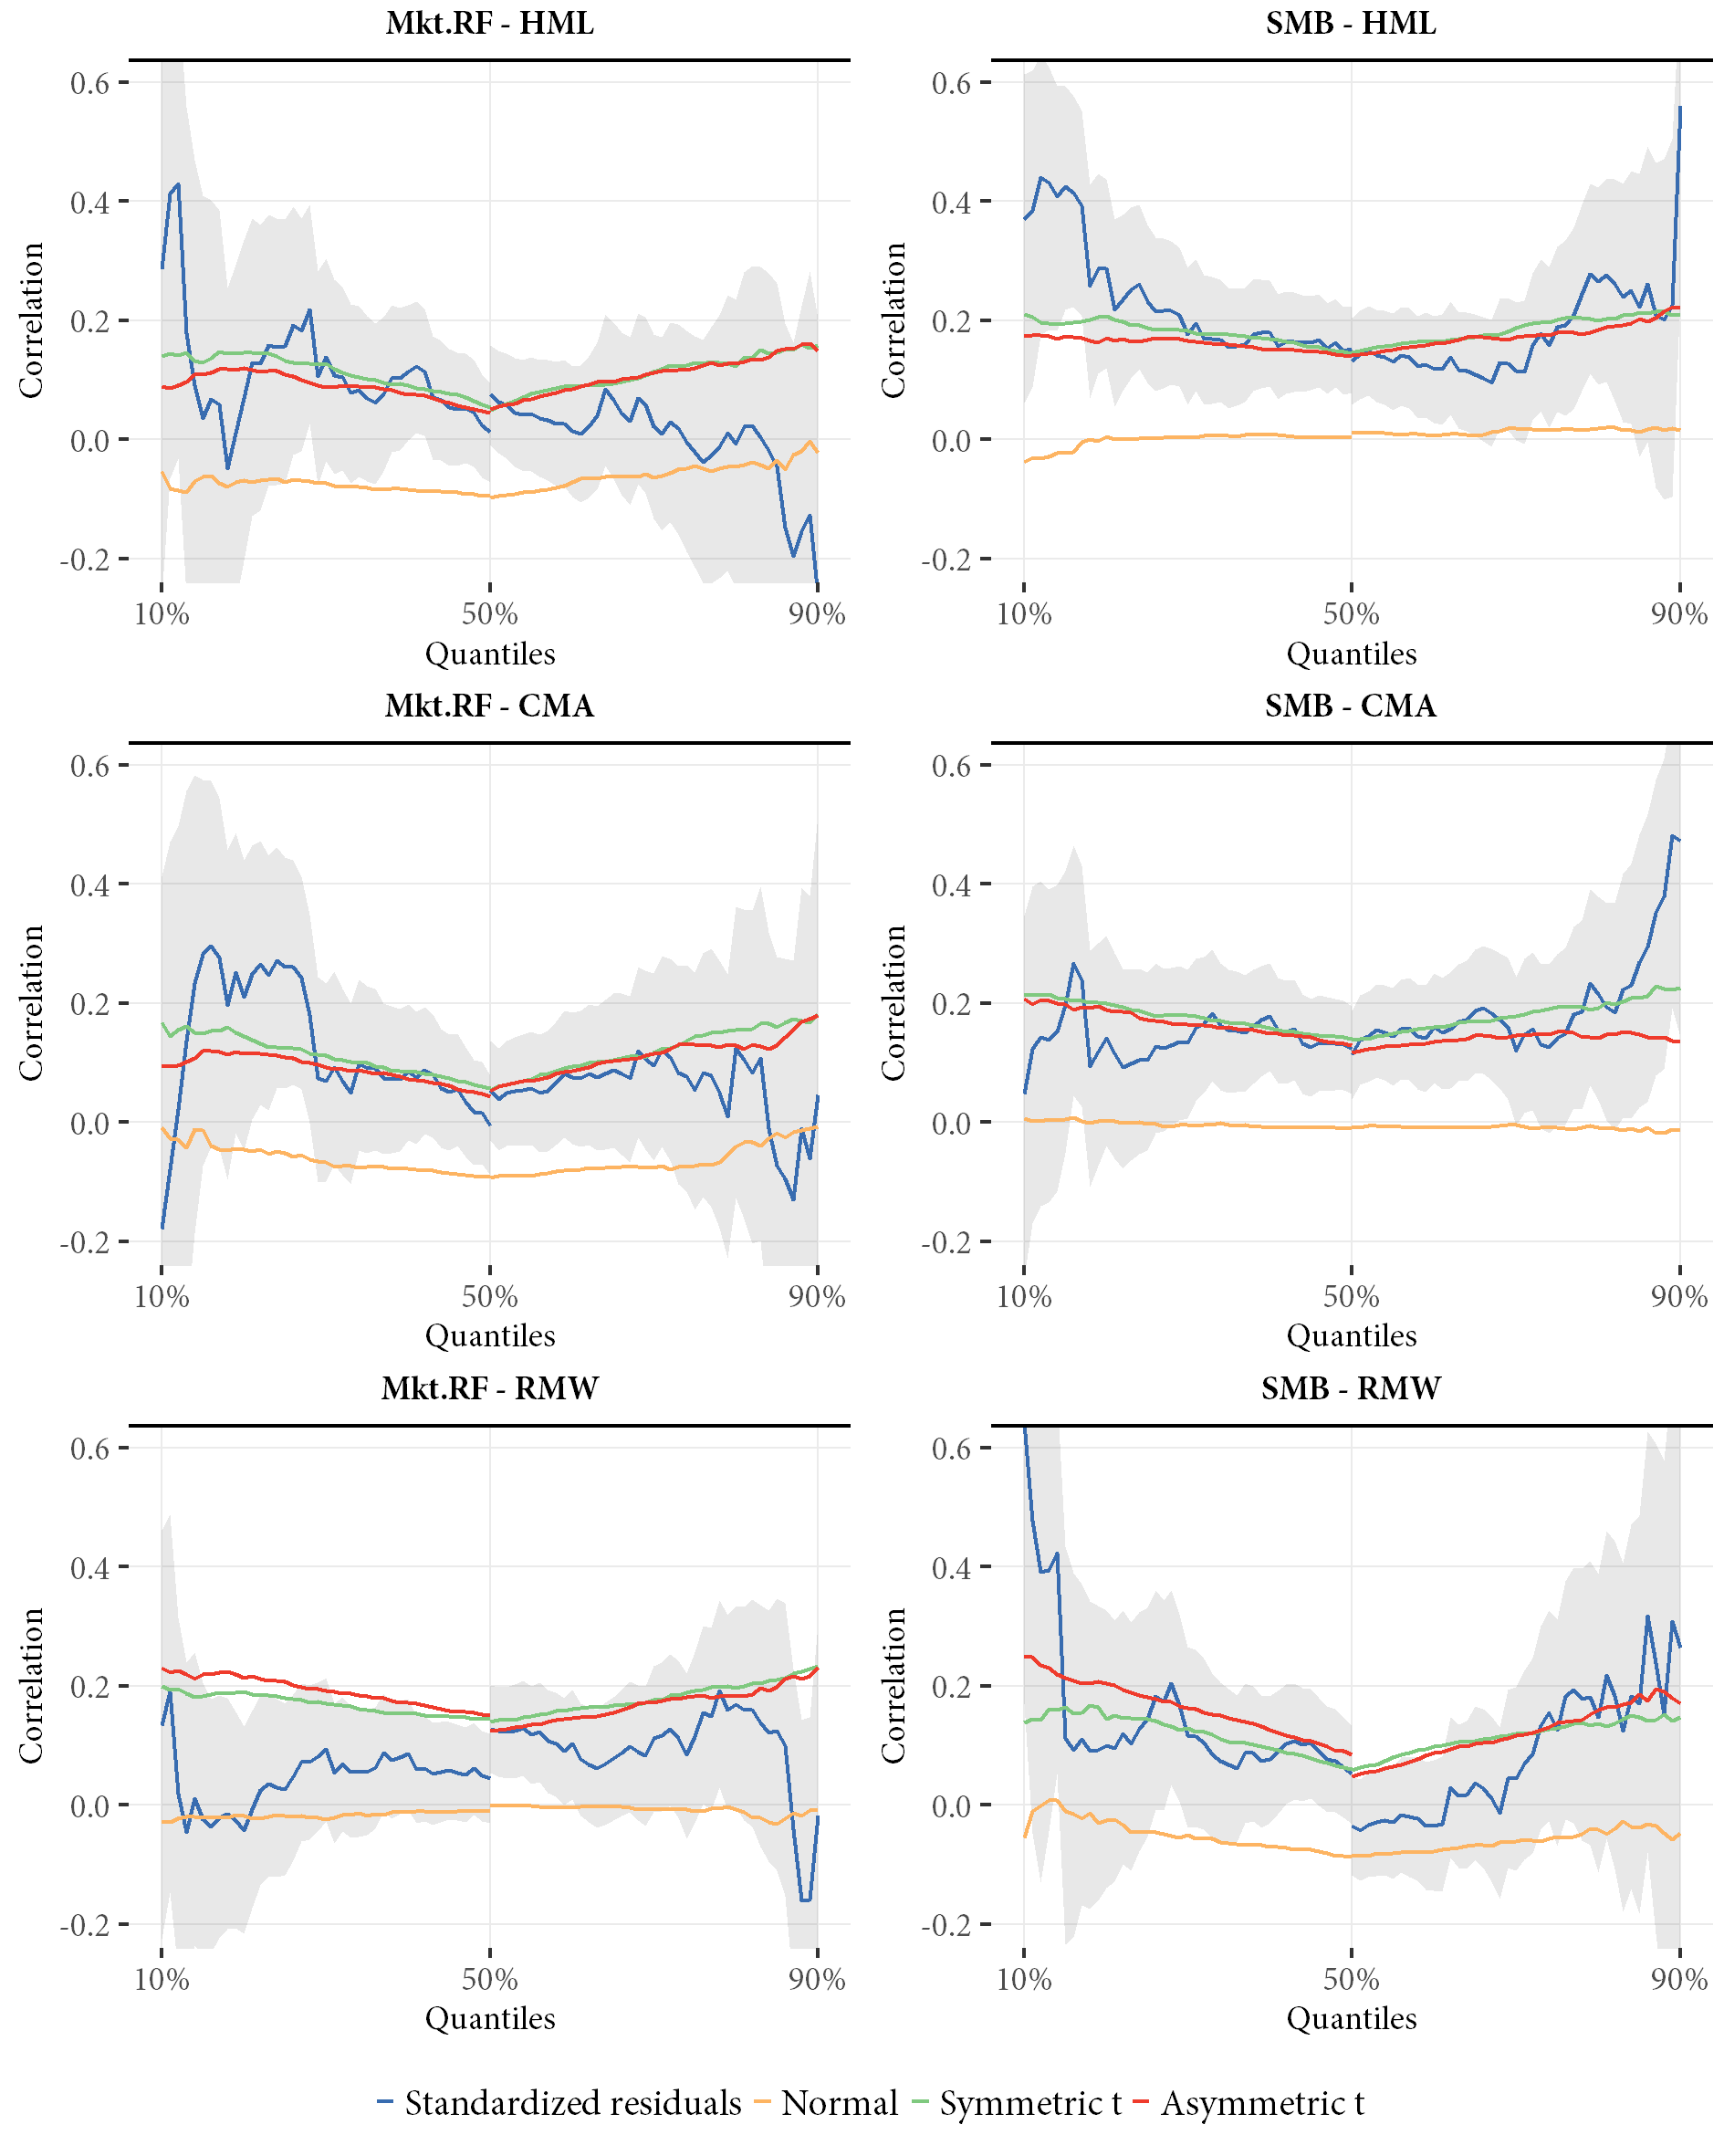
\includegraphics[scale=1]{graphics/threshold_simulated_1.png}  
  \footnotesize
  \caption{Threshold correlations of standardized residuals from the constant copulas}

  \begin{longcaption}
    Threshold correlations of simulated constant copulas, compared to ARMA-GARCH standardized residuals (95\% confidence bounds taking the ARMA-GARCH models as given). The simulated threshold correlations are based on 250,000 simulated returns each. ARMA-GARCH models based on empirical weekly data 1963--2016.
  \end{longcaption}
  \label{fig:threshold_simulated1}
\end{figure}
\pagebreak
\begin{figure}[!ht]
  \ContinuedFloat
  \centering
  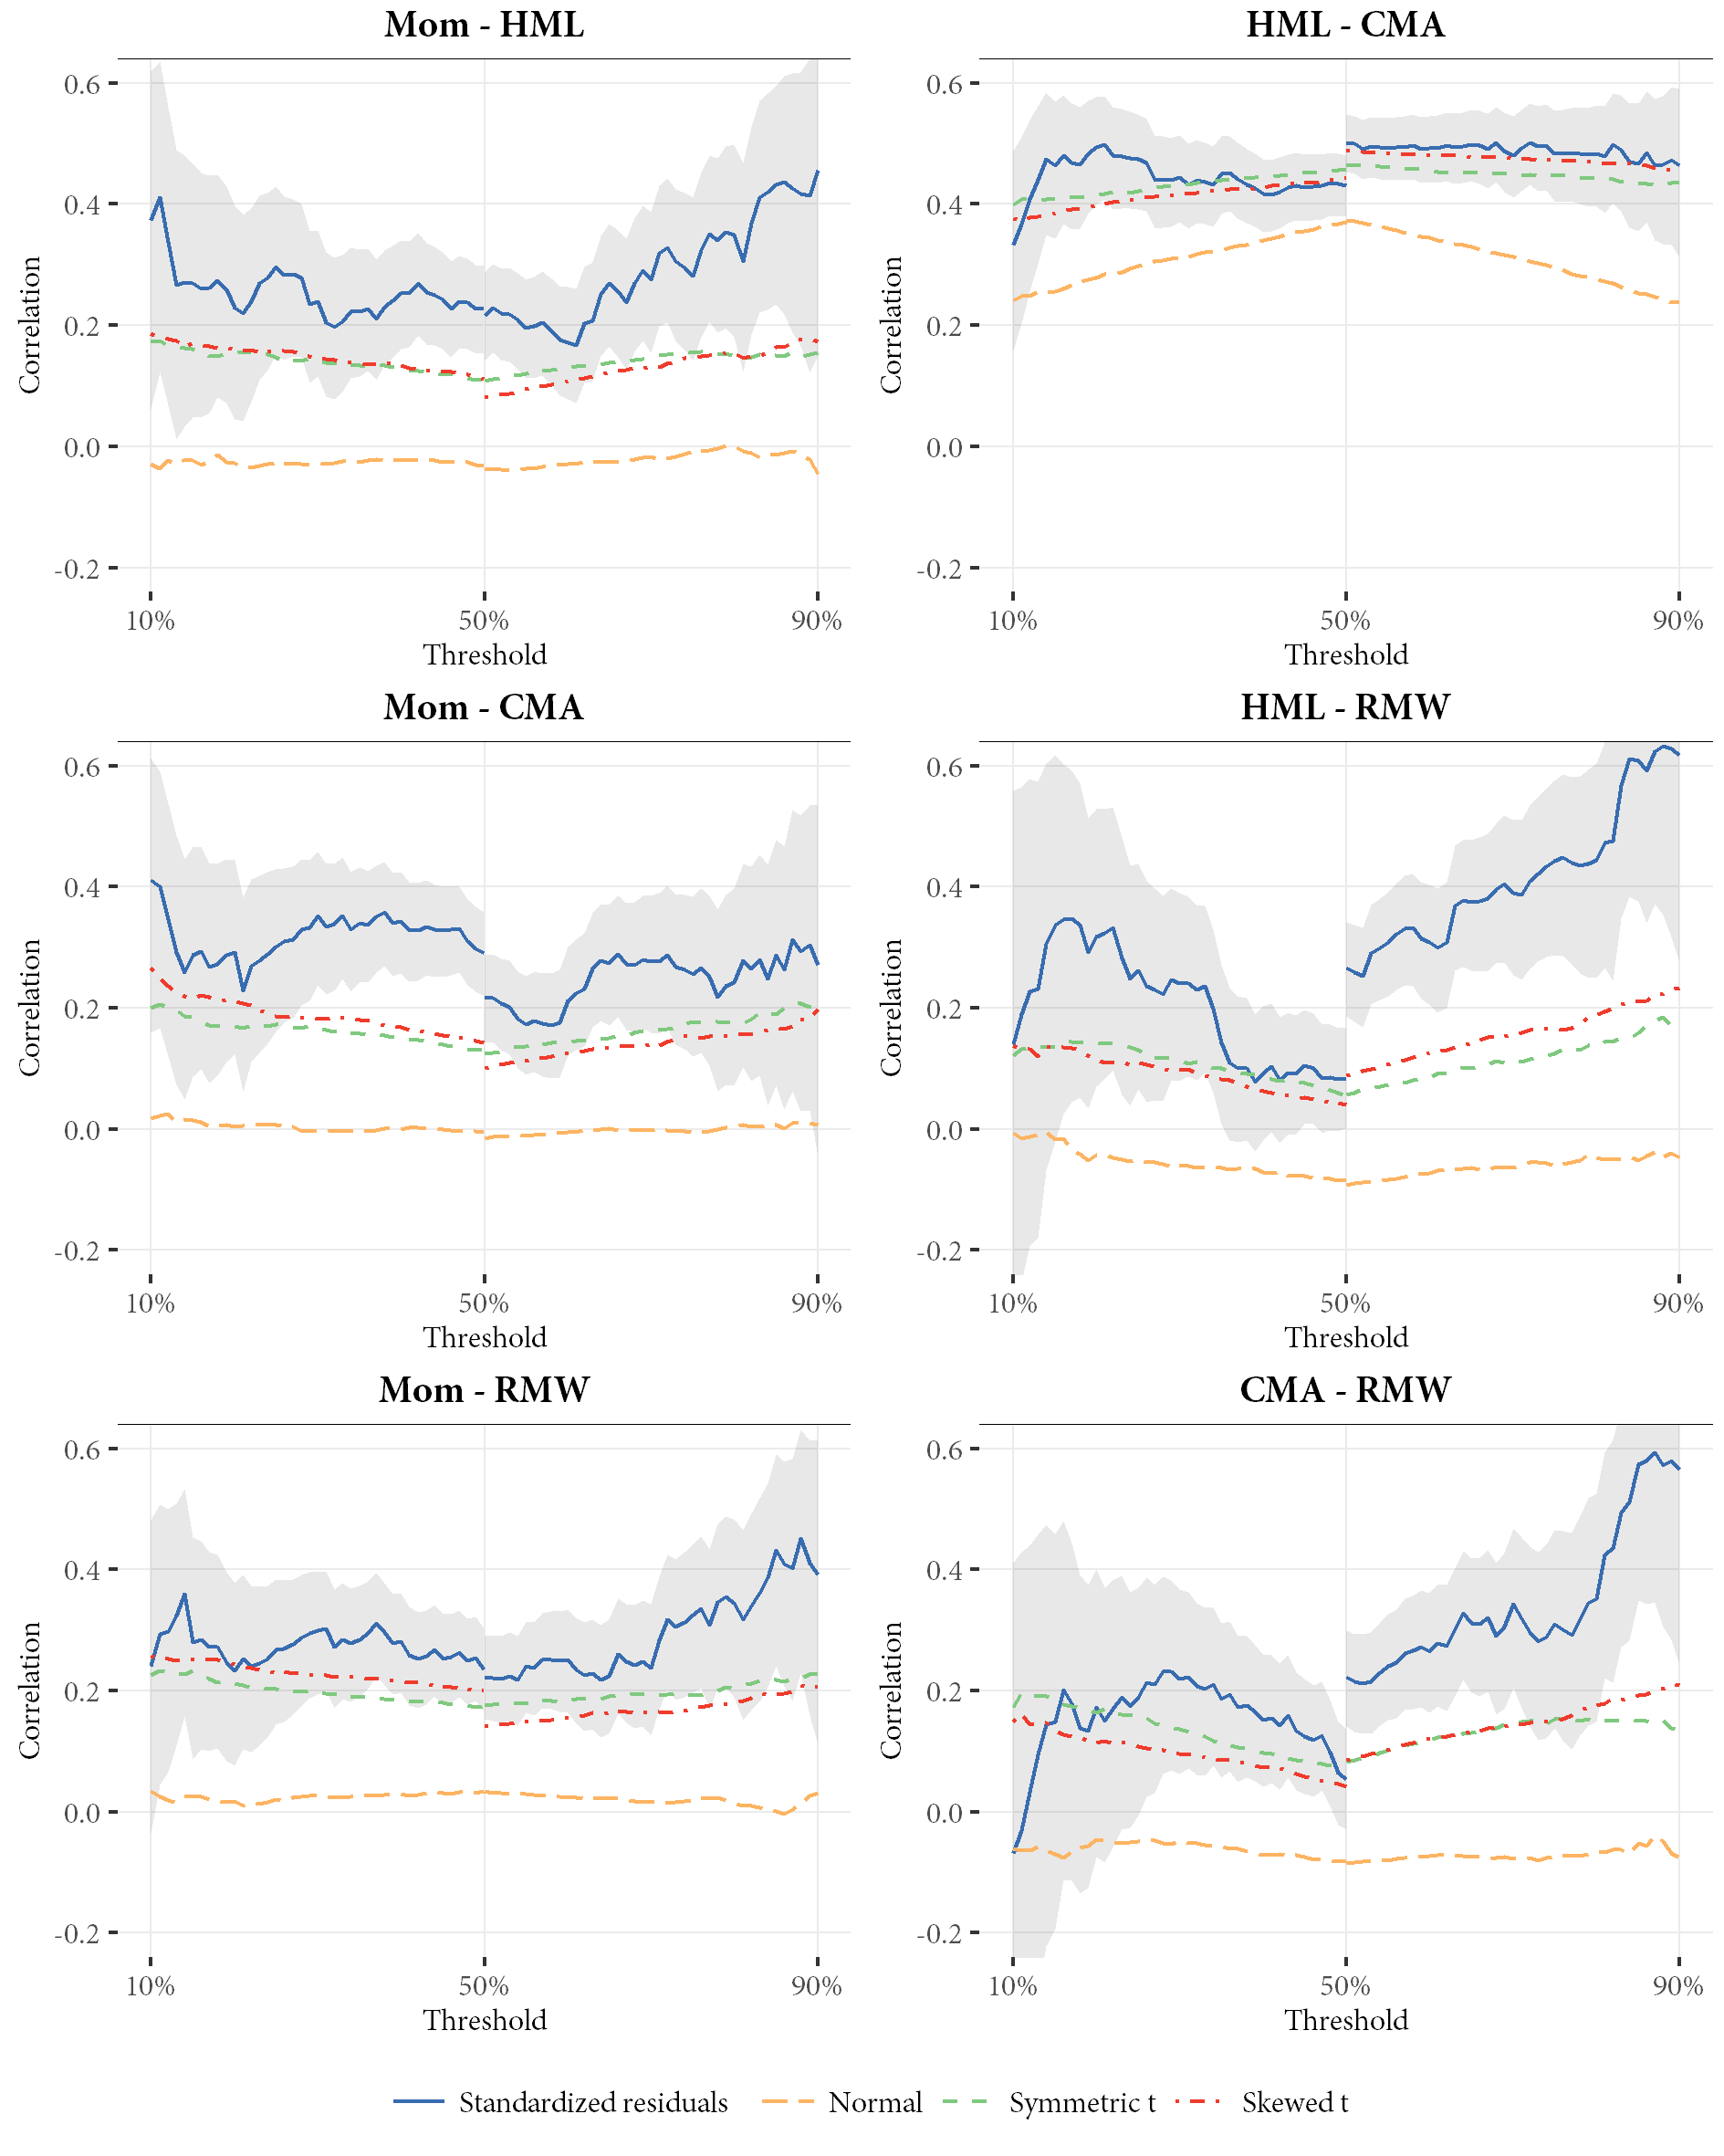
\includegraphics[scale=1]{graphics/threshold_simulated_2.png}  
  \footnotesize
  \caption{Threshold correlations of standardized residuals from the constant copulas (cont.)}
\end{figure}
\pagebreak

First, we note that for most factors, the normal copula is the far away from generating threshold correlations that correspond to the empirical distribution around the median. This is highly expected, as the normal copula does not generate tail dependence, and hence the need for the Student's \textit{t} based copula models. The symmetric \textit{t} and asymmetric \textit{t} copulas better capture the threshold correlations, as the fatter tails of the Student's \textit{t} distribution allows for tail dependence. For example, note how the normal copula generates negative threshold correlations for both the Mom--HML and RMW--HML asset pairs, while the Student's \textit{t} based copulas are much closer to the higher values in the data. On the other hand, the Student's \textit{t} based copulas sometimes seem to overshoot the empirical threshold correlation, as in the Mkt.RF--RMW asset pair.

Second, we find that the skewed Student's \textit{t} generates some asymmetry around the median, which can be seen most clearly for the Mom--RMW and RMW--HML asset pairs. The generated asymmetry does, however, appear to be too small to capture the features of the data.

In conclusion, comparing threshold correlations from empirical data and simulated data shows that the constant copula specifications capture some of the tail dependence.\footnote{Note that, in order to make the threshold correlation comparison valid, we use the constant copula specifications. The dynamic version is still the workhorse for all continued analysis in the mean-variance and diversification benefit sections.} Although the Student's \textit{t} and skewed Student's \textit{t} results do not align perfectly with the data, they constitute clear improvements to the normal copula in modeling tail dependence. We observe that the copula seems to lack flexibility to simultaneously generate all the asymmetries in tail dependence. This is quite expected, as the Student's \textit{t} copula only has one degree of freedom parameter that controls the fatness of tails, and the skewed Student's \textit{t} copula only has one skewness parameter for each series. This imposes limits on how strongly the model can express fat tails or asymmetries between factors A and B and simultaneously express other fat tails or asymmetries (or lack thereof) between factors A and C. For a collection of six factors with heterogenous dependence, this is even harder. This is a clear limitation of our quite parsimonious multivariate distribution copula approach. In this regard, vine copulas that allow for unique bivariate copula specifications, as discussed in \autoref{sub:05_01_choosing}, could be the solution.

Although imperfect, the multivariate copula modeling of tail dependence could constitute a significant improvement to alternatives, especially in the field of risk management, where understanding of tail events is paramount.

\subsubsection{Rolling correlations in the dynamic copula}

In-sample, we simulate 10,000 standardized residuals for each week from the estimated dynamic symmetric Student's \textit{t} copula model, and compute the rolling 52-week correlations. This is done to ascertain ourselves that the chosen copula specification does in fact capture the time-variation in correlations. The comparison is made between standardized residuals from the simulated copula model and standardized residuals from the ARMA-GARCH model of univariate series. If satisfactory, the rolling correlations of the copula model and the ARMA-GARCH univariate models will be roughly the same.

\begin{figure}[!ht]
  \centering
  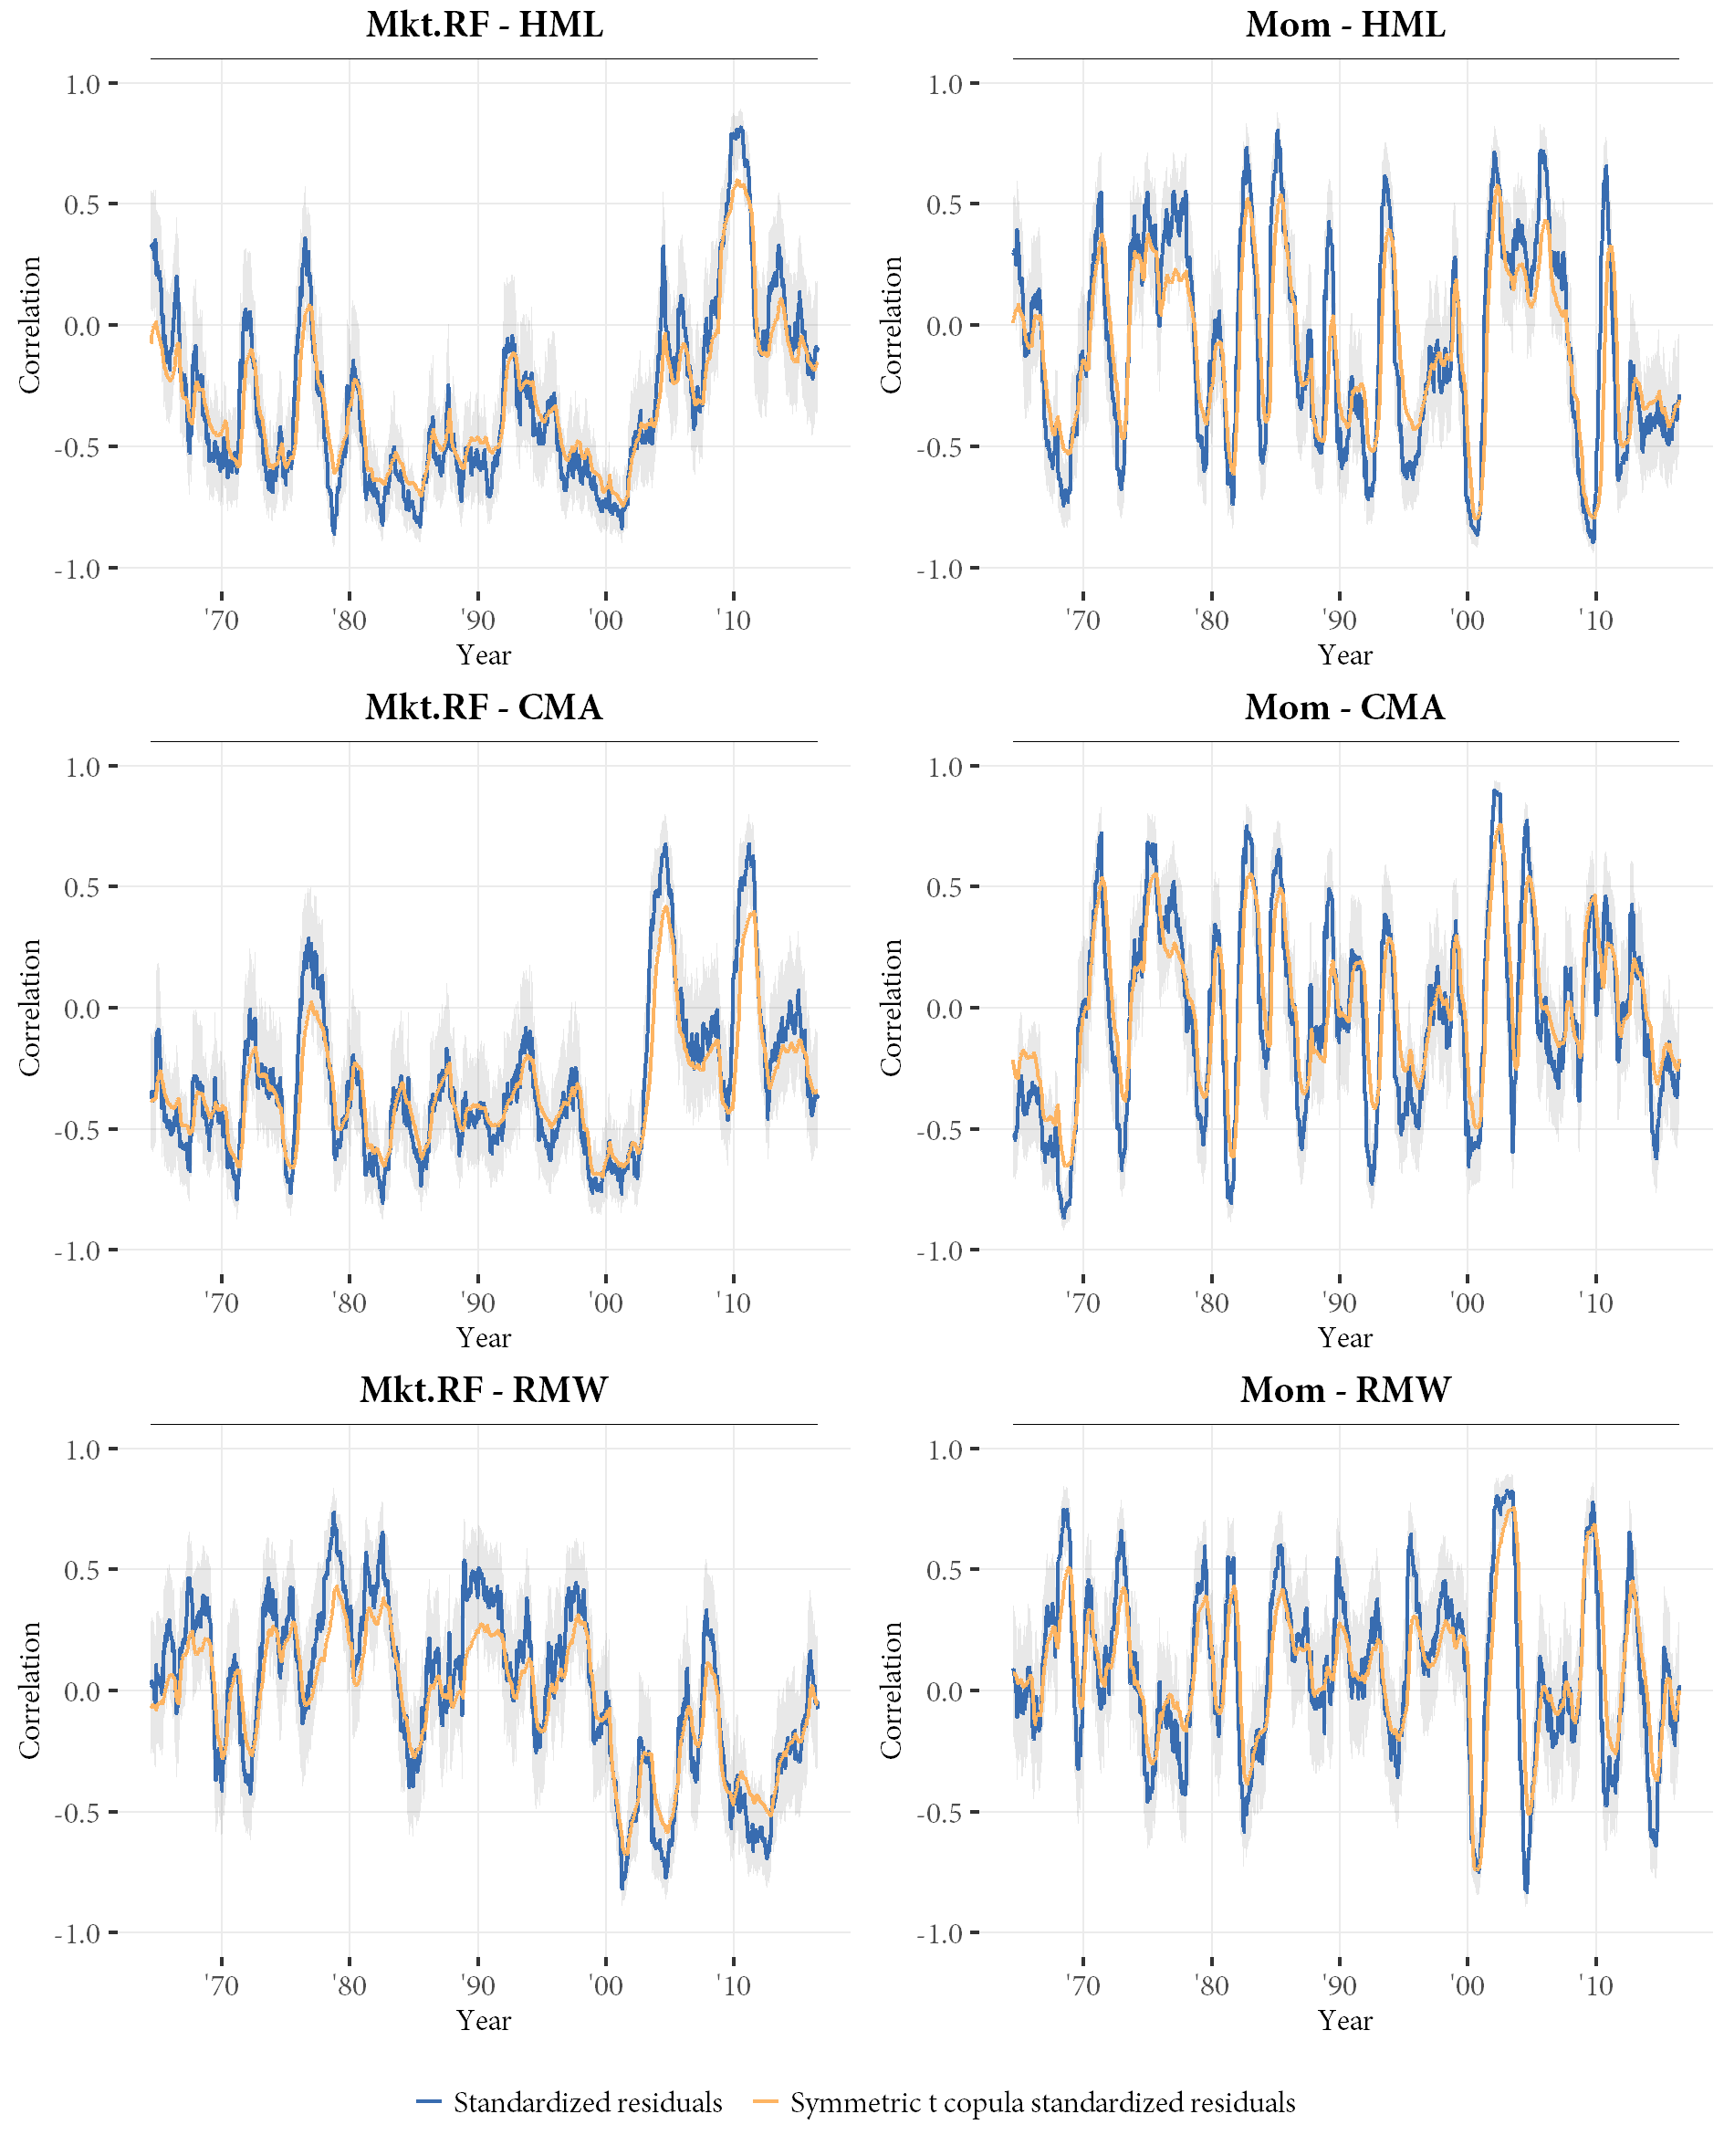
\includegraphics[width=\textwidth]{graphics/rolling_simulated1.png}
  \footnotesize
  \caption{Rolling correlations of standardized residuals from the dynamic copula}

  \begin{longcaption}
    Rolling correlations of the simulated dynamic symmetric \textit{t} copula compared to rolling correlations on ARMA-GARCH residuals. 95\% confidence bounds taking the ARMA-GARCH models as given. The simulated rolling correlations are based on 10,000 simulations each week. ARMA-GARCH models based on empirical weekly data 1963--2016.
  \end{longcaption}
  \label{fig:rolling_simulated}
\end{figure}
\begin{figure}[!ht]
  \ContinuedFloat
  \centering
  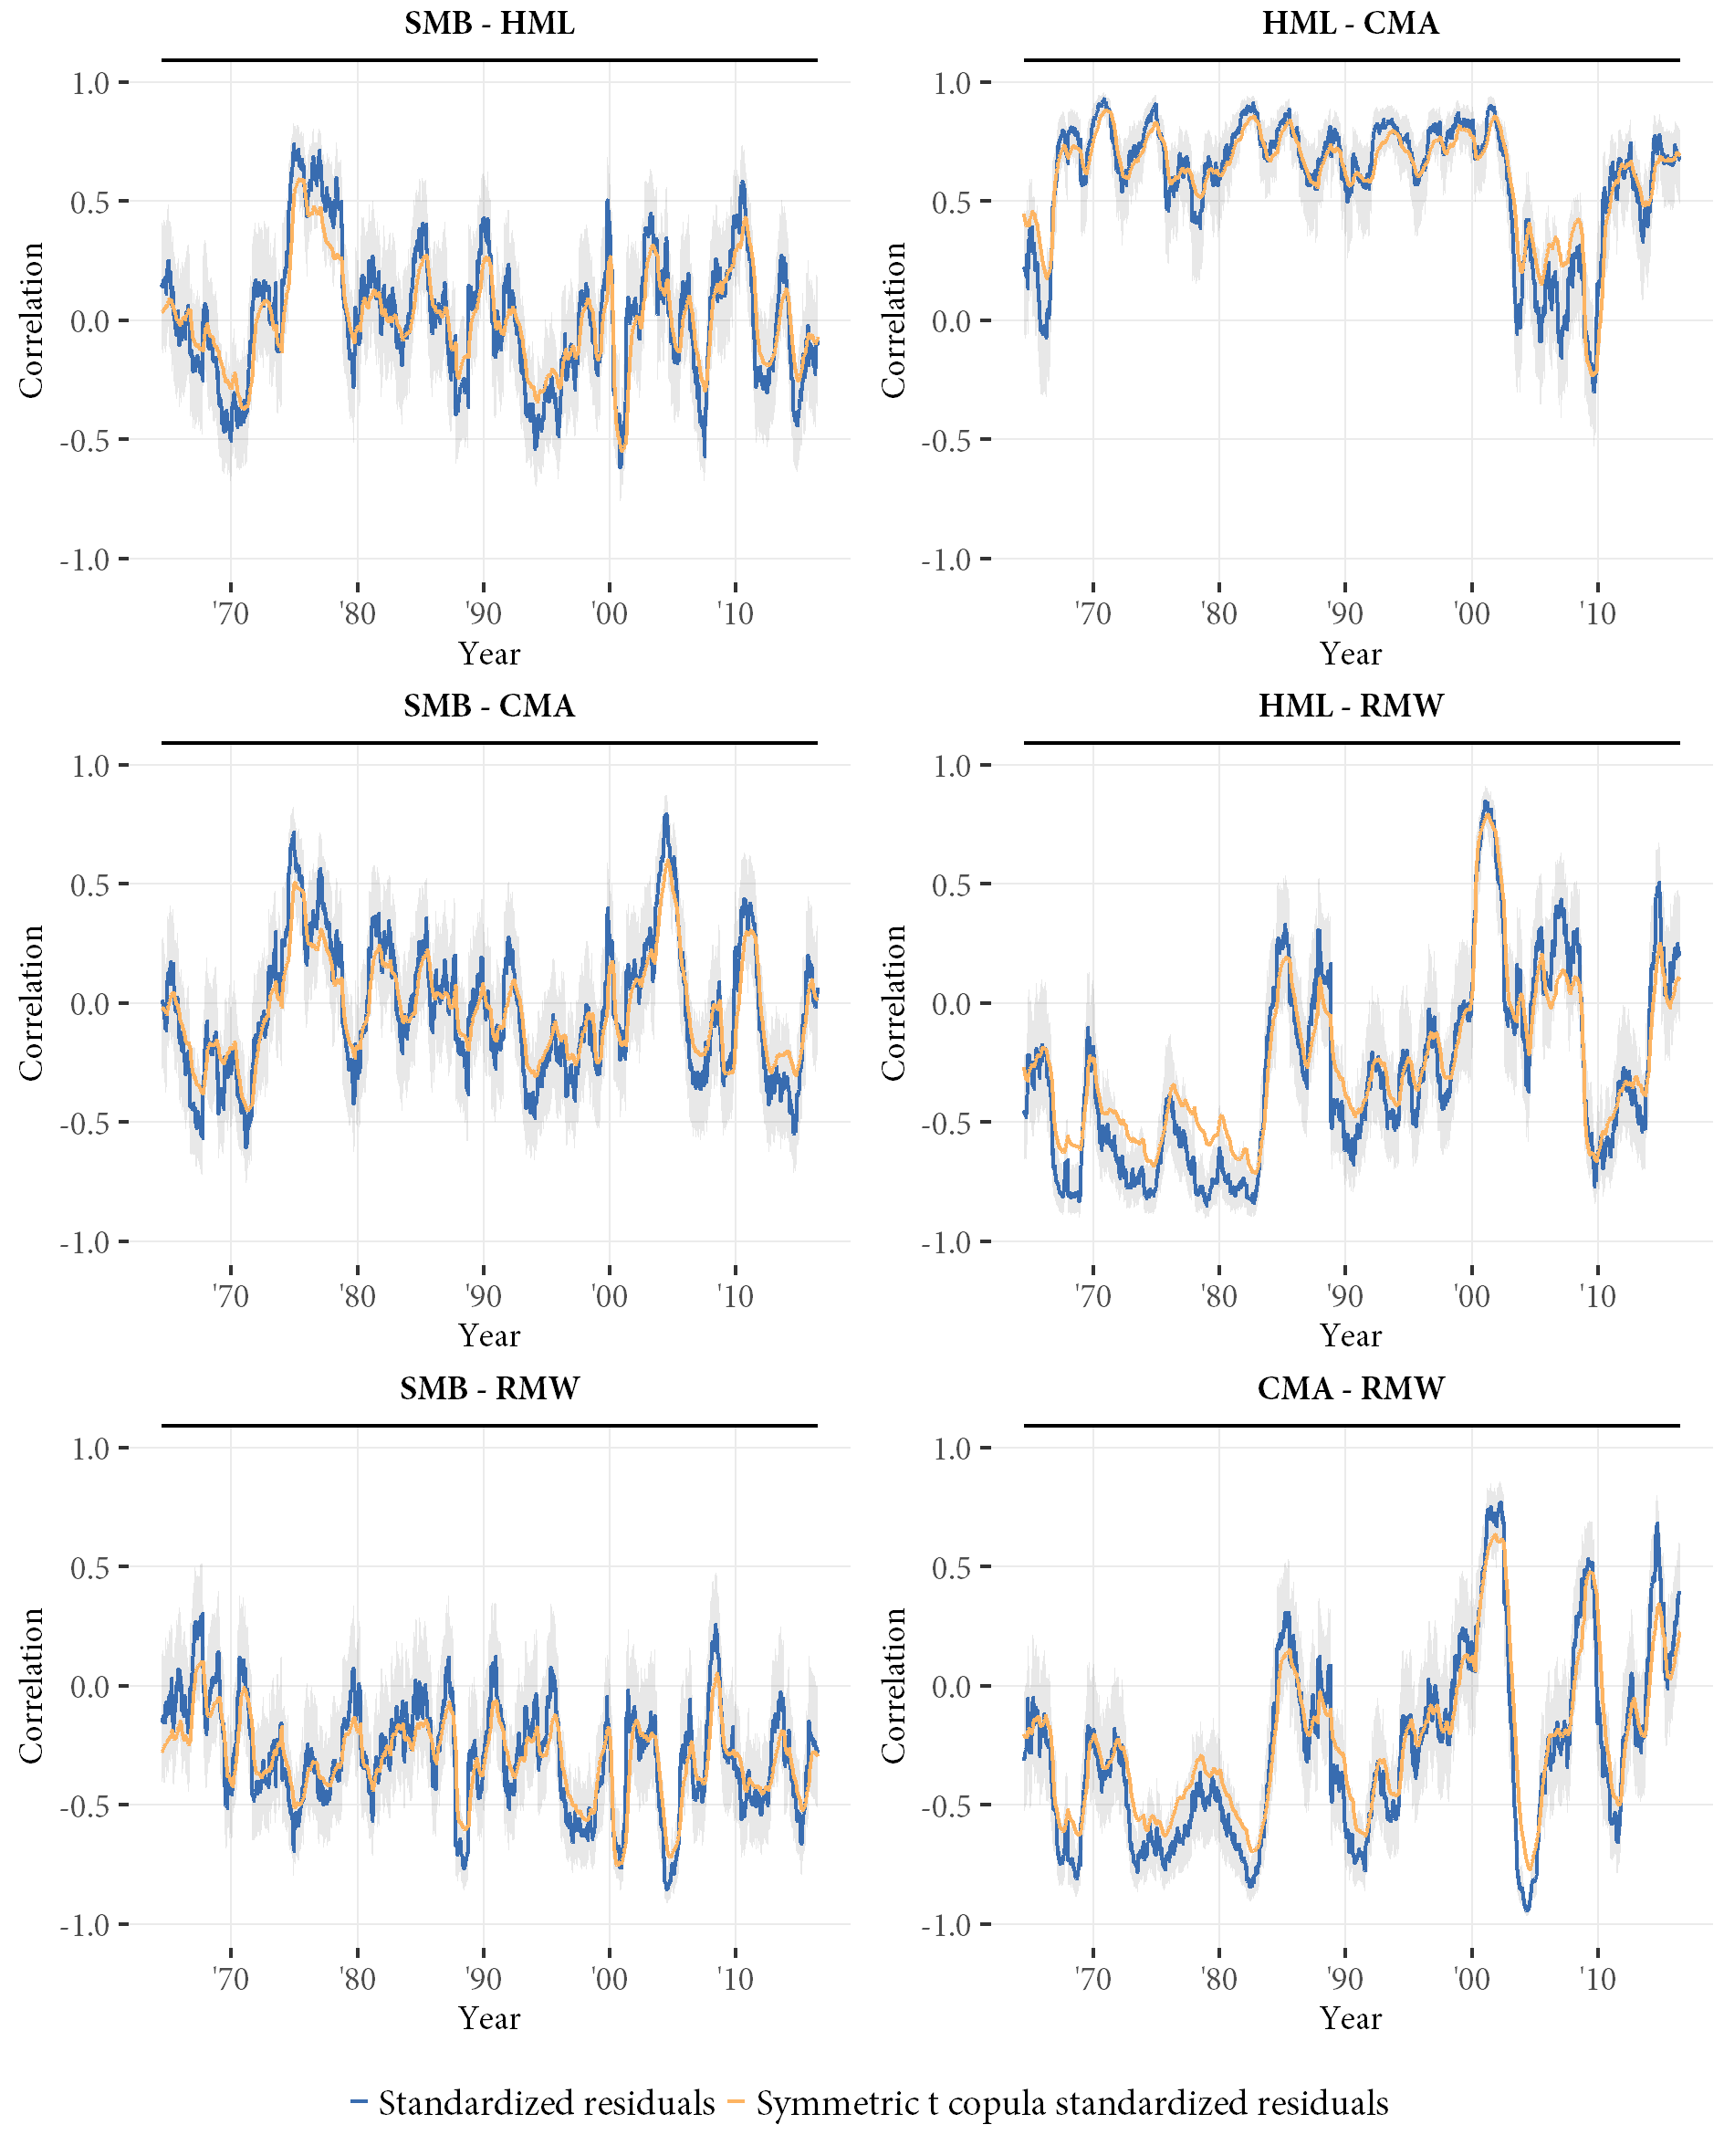
\includegraphics[width=\textwidth]{graphics/rolling_simulated2.png}
  \footnotesize
  \caption{Rolling correlations of standardized residuals from the dynamic copula (cont.)}
\end{figure}

While we do not get a perfect overlap, the copula model generates similar time-varying correlations. When there are large swings, however, the model does not always have enough amplitude. We conclude that the model captures the dynamic features well.